%%%%%%%%%%%%%%%%%%%%%%%%%%%%%%%%%%%%%%%%%%%%%%%%%%%%%%%%%%%%%%%%%%%%%%%%%%%%
%% Chapter 5
%%Indian Institute of Information Technology Kalyani
%% All rights are reserved.
%%%%%%%%%%%%%%%%%%%%%%%%%%%%%%%%%%%%%%%%%%%%%%%%%%%%%%%%%%%%%%%%%%%%%%%%%%%%

\chapter{Technical Implementation}
\label{chp5}

Designing a Central Bank Digital Currency (CBDC) system goes beyond simply digitizing cash. It requires creating a secure, efficient, scalable, and inclusive ecosystem capable of serving a diverse population like India's. This chapter outlines the technical blueprint for how such a system could be developed and implemented. While this work does not present a fully functional prototype, it provides a detailed analysis of the tools, architecture, and technologies essential to realizing an operational CBDC framework for India.

\section{Tools and Frameworks Considered}
Developing a CBDC involves selecting technologies that can ensure security, scalability, interoperability, and accessibility. Based on the unique demands of implementing a national-level digital currency, the following tools and frameworks have been evaluated:

\subsection*{Distributed Ledger Technology (DLT)}
DLT ensures secure and tamper-resistant transaction records. The following platforms are considered suitable:
\begin{itemize}
    \item \textbf{Hyperledger Fabric:} Permissioned, enterprise-grade blockchain ideal for regulated environments.
    \item \textbf{Ethereum:} A public blockchain platform with broad adoption and smart contract support.
    \item \textbf{Corda:} Tailored for financial institutions, supporting privacy and transaction control.
\end{itemize}

\subsection*{Simulation Tools}
Simulating system behavior before deployment helps evaluate robustness under various conditions. Tools include:
\begin{itemize}
    \item \textbf{MATLAB:} Useful for modeling control systems and network behavior.
    \item \textbf{AnyLogic:} Allows detailed simulation of transaction flows, failures, and network loads.
\end{itemize}

\subsection*{Wallet SDKs and APIs}
User interaction relies heavily on mobile interfaces. Development tools include:
\begin{itemize}
    \item \textbf{UPI APIs:} For secure and instantaneous fund transfers.
    \item \textbf{Flutter and React Native:} Enable cross-platform mobile wallet development.
\end{itemize}

\section{Architecture Overview}
The CBDC architecture is designed as a hybrid model, combining centralized governance with decentralized access. Key components include:
\begin{itemize}
    \item \textbf{Central Bank (RBI):} Responsible for issuance, policy control, and system oversight.
    \item \textbf{Commercial Banks and PSPs:} Serve as intermediaries, distributing CBDC and managing user accounts.
    \item \textbf{End Users:} Citizens, merchants, and government bodies interact with the CBDC via wallets.
\end{itemize}

This layered approach retains centralized security and trust while distributing operational workload across financial intermediaries.

\begin{figure}[H]
\centering
% \fbox{\includegraphics[width=0.8\textwidth]{Figure/chp5/architecture-diagram.png}}
\caption{Proposed Architecture of the CBDC System}
\label{fig:chp5-architecture}
\end{figure}

\section{Data Flow and Process}
A standard transaction in the CBDC system follows these steps:
\begin{enumerate}
    \item \textbf{User Authentication:} Verified through Aadhaar-based eKYC, biometric data, or device-level checks.
    \item \textbf{Transaction Initiation:} Users scan QR codes or enter recipient details to initiate payments.
    \item \textbf{Ledger Update:} Transactions are recorded on the distributed ledger, ensuring transparency and immutability.
    \item \textbf{Transaction Confirmation:} Both sender and receiver receive real-time confirmation of the transfer.
\begin{figure}
    \centering
    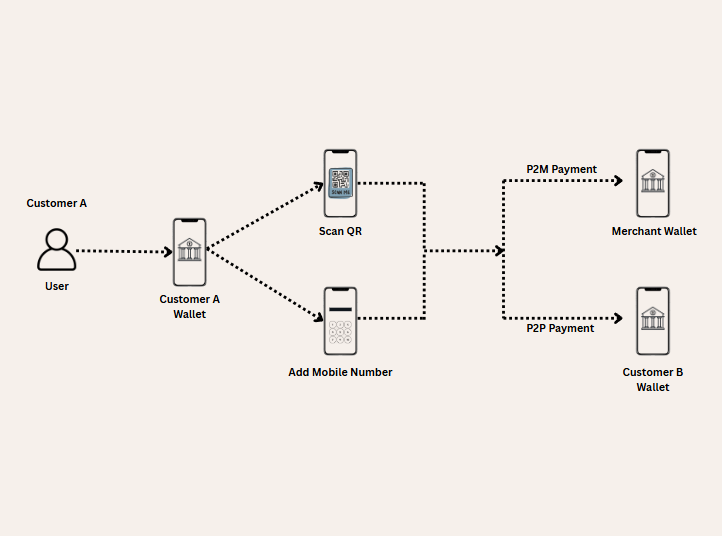
\includegraphics[width=0.9\linewidth]{chp5img1.png}
    \caption{Transaction by User Flowchart}
    \label{fig:enter-label}
\end{figure}
\end{enumerate}
This end-to-end flow ensures security, speed, and integrity in every transaction.

\section{Use Case Scenarios}
CBDC has broad applicability. Key scenarios include:
\begin{itemize}
    \item \textbf{Retail Transactions:} Instant payments in physical and online stores.
    \item \textbf{Peer-to-Peer Transfers:} Seamless fund movement between individuals.
    \item \textbf{Government Payments:} Direct Benefit Transfers (DBT) and subsidies without intermediaries.
    \item \textbf{Offline Usage:} Payments in no-network zones via NFC cards or QR-enabled devices.
\end{itemize}

\section{Security Considerations}
Given its financial nature, the CBDC system integrates multiple security layers:
\begin{itemize}
    \item \textbf{Double-Spending Prevention:} Unique token IDs ensure each unit is spent only once.
    \item \textbf{Cryptographic Security:} Public-private keys secure all wallet operations.
    \item \textbf{Counterfeit Protection:} Digital watermarking verifies currency authenticity.
    \item \textbf{Infrastructure Resilience:} Load balancing, backups, and failover systems ensure availability.
\end{itemize}

\section{Conclusion}
Implementing a CBDC at a national scale is an ambitious but transformative goal. It requires the fusion of advanced technologies with the stability and trust of traditional finance. The proposed hybrid system architecture, powered by a robust technology stack, enables secure, efficient, and inclusive access to digital money.

Although this chapter presents a conceptual design rather than a functional system, it offers a practical foundation upon which India can build its CBDC. Future steps involve prototyping, pilot testing, and policy alignment to transition from theoretical models to real-world applications, ensuring that digital currency becomes a reality for every citizen---regardless of geography or connectivity.
